\lesson{Quantum Theory and Quantum Numbers}
\subsection{Flaw with Rutherford's Model}
\begin{bulleted-list}
    \item Rutherford believed that the electrons orbited around the nucleus like planets
    \item Only problem was that they should be emitting energy, meaning that they would eventually
        collapse into the nucleus. See Figure \ref{fig:rutherford-model-flaw}
    \item This would leave the atom unstable, so chemists knew this was not the case
\end{bulleted-list}

\begin{figure}[ht!]
    \centering
    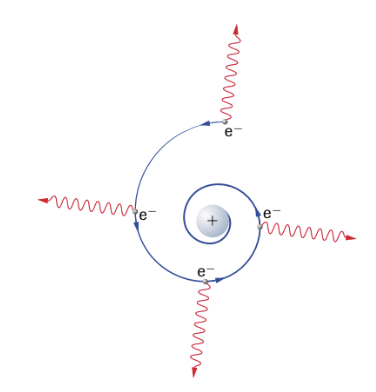
\includegraphics[width=0.4 \textwidth]{../figures/rutherford-model-flaw.png}
    \caption{According to Rutherford's model, an obiting electron should continuously emit
            electromagnetic radiation, losing energy, and collapse the atom. The evidence is to the
            contrary}
    \label{fig:rutherford-model-flaw}
\end{figure}

\subsection{Atomic Spectra}
\begin{bulleted-list}
    \item Robert Bunsen and Gustav Kirchhoff worked together to invent the \textbf{spectroscope}.
        See Figure \ref{fig:spectroscope}
    \item The spectroscope forms the basis of an analytic method called \textbf{spectroscopy}
    \item Bunsen and Kirchhoff studied the spectra of chemicals, especially elements, heated in
        a Bunsen burner flame, and the spectrum of the Sun. They discovered that an element not
        only produced a characteristic flame colour but, on closer examination through a
        spectroscope, also produced a \textbf{bright-line spectrum} that was characteristic of
        the element
    \item This techique was used to catalogue known elements and when a new spectrum was found,
        the spectrum was used as evidence of a new element
    \item The elements \textbf{cesium} and \textbf{rubidium} were discovered within a year of
        the invention of spectroscopy
    \item \textbf{Spectroscopy:} a tehcnique for analyzing spectra; the spectra may be visible
        light, infrared, ultraviolet, X-ray, and other types
    \item \textbf{Bright-line spectrum:} a series of bright lines of light produced or emitted by
        a gas excited by, for example, heat or electricity
    \item \textbf{Note:} spectroscopes may separate the light by using a prism, or a
        \textbf{diffraction grating}. The most modern, compact, and inexpensive school spectrometers
        use a diffraction grating
\end{bulleted-list}

\begin{important}
    Different elements have different spectrums because they have different number of protons,
    and different arrangement of electrons. The differences in spectra reflects the differences
    in the amount of energy that the atoms absorb or give off when their electrons move between
    energy levels. Hence, this is an effective technique in identifying new elements.
\end{important}

\begin{figure}[ht!]
    \centering
    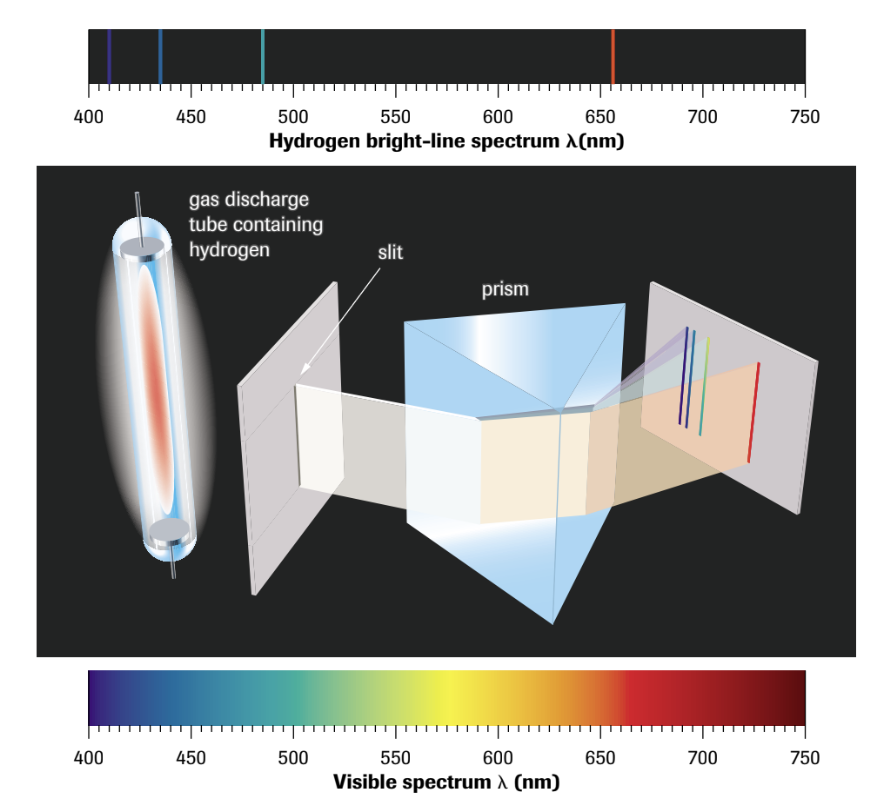
\includegraphics[width=0.9 \textwidth]{../figures/spectroscope.png}
    \caption{Light from a source of light is passed through slits to form a narrow beam. This beam
            is split into its components by the prism to produce a series of coloured lines. The visible region
            of the hydrogen spectrum includes four coloured lines at the wavelengths shown by the scale}
    \label{fig:spectroscope}
\end{figure}

\begin{bulleted-list}
    \item Around 1814, \textbf{absorption} or \textbf{dark-line spectra} were investigated by
        Joseph von Fraunhofer
    \item Kirchhoff, among others, was able to show in the 1860s that dark lines in an element's
        spectrum were in the same position as the bright lines in the spectrum of the same element.
        See Figure \ref{fig:dark-line-spectrum}
    \item This provided a powerful tool to determine the composition of gases far away in the
        universe. When light passes through a gas, for example, the atmosphere around the Sun,
        some light is absorbed by the atoms present in the gas
\end{bulleted-list}

\begin{figure}[ht!]
    \centering
    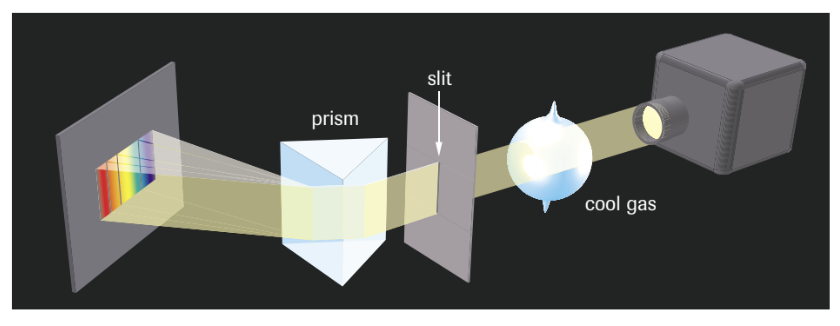
\includegraphics[width=0.9 \textwidth]{../figures/dark-line-spectrum.png}
    \caption{If you start with a complete colour spectrum of all possible colours, then pass this
            light through a gas and analyze what is left, you get a dark-line spectrum; in other words,
            the complete spectrum with some lines missing.}
    \label{fig:dark-line-spectrum}
\end{figure}

\subsection{Bohr's Model}
\begin{bulleted-list}
    \item Bohr reasoned that if the light released or absorbed from an atom was quantized, then the
        energy of the electron inside the atom must also be quantized. In other words, an electron
        can only have certain energies. The simplest arrangement would be a planetary model with
        each electron orbit at a fixed distance with a fixed energy
    \item Electrons do move in a circular orbit around the nucleus, with the motion described
        by classical physics
    \item Electrons have only a \textbf{fixed set of allowed orbits}, called \textbf{stationary states}.
        Stationary in the sense that the energy is constant
        As long as an electron remains in its orbit, its energy is constant and gives off no energy
    \item An electron can only pass from one allowed orbit to another. That is, electrons cannot
        lie between orbits
    \item Bohr observed the spectrum lines when observing hydrogen. The non-continuous
        colours suggested only certain energies were released. See Figure \ref{fig:hydrogen-spectrum-lines}
    \item There are two states for electrons:
        \begin{enum}
            \item \textbf{Ground state:} the ``expected'' arrangement of electrons. This is because
                this is the lowest amount of energy the electrons can possess
            \item \textbf{Excited state:} When an electron temporarily occupies an energy state higher
                than its ground state--it is moving between energy levels. The more energy the 
                electron absorbed, the higher the energy levels the electrons can move to.
                Eventually, the electron returns back to the ground state, releasing energy
                in the form of \textbf{photons}
            \item In other words, under normal circumstances, in the ground state, the electrons
                occupy the energy levels which they should--the electron in hydrogen is in the first
                energy level. But, if we were to add energy to hydrogen, the excited state of
                the electron could occupy the second, third, or even fourth energy level. Once
                the energy is released, the electron will come back down to the ground state
            \item The dark line spectrum is what we observe when electrons gain energy and move
                to higher energy levels. These dark lines indicate the amount of energy that was
                absorbed when they moved
        \end{enum}
\end{bulleted-list}

\begin{figure}[ht!]
    \centering
    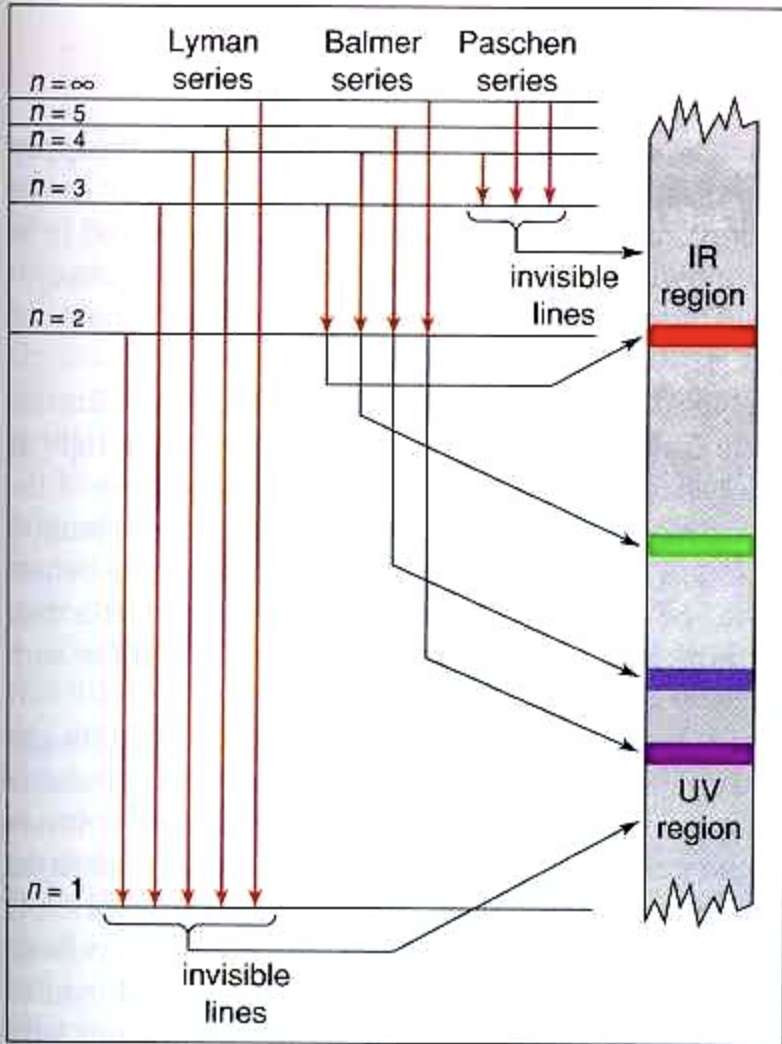
\includegraphics[width=0.6 \textwidth]{../figures/hydrogen-spectrum-lines.png}
    \caption{Because there are so many atoms, and thus a lot of electrons, in a sample of hydrogen 
            gas, there would be a continuous spectrum and not individual lines. These lines indicate
            that energy is released in quanta and not continuous}
    \label{fig:hydrogen-spectrum-lines}
\end{figure}

\subsection{Quantum Theory}
The energy of a photon of electromagnetic radiation is \textbf{proportional} to its frequency,
not to its intensity/brightness as had been believed up to that time. This is used to derive
the Planck equation
\[
    E=h\nu
\]
Where $E$ is the energy, $h=6.63\times10^{-34}\,\si{J.s}$, the Planck constant, and $\nu=$ the
frequency of the wave.\\

There are 4 distinct numbers, coupled together as coordinates, to represent the location of
an electron in an atom. This is called \textbf{quantum numbers}

\begin{enum}
    \item \textbf{Principle quantum number:} this represents the energy level in the atom.
        Denoted by $n$, it has the range
        \begin{align*}
            \text{theoretical: }&[1,\,\infty)\\
            \text{practical: }&[1,\,7]\quad\text{7 periods on the periodic table}
        \end{align*}
        The theoretical number of total electrons given a quantum number is $2n^2$. This is the 
        only quantum number that matters, because the other numbers are considered ``labels''
    \item \textbf{Secondary quantum number:} this represents the shape of the orbital.
        Denoted by $\ell$, it has the range 
        \begin{align*}
            \text{theoretical: }&[0,\,n-1]\\
            \text{practical: }&[0,\,4]\\
            \text{notation }&(s,\,p,\,d,\,f)
        \end{align*}
        \begin{bulleted-list}
            \item \textbf{Arnold Sommerfeld} expanded on Bohr's theory when he realized many
                of the lines Bohr observed were actually \textbf{multiple lines} very tighly
                together
            \item Sommerfield decided to split energy levels into \textbf{sub-energy} levels,
                having only slightly different energies. This is how they derived the secondary 
                quantum number
        \end{bulleted-list}
    \item \textbf{Magnetic quantum number:} this represents the orientation of the orbital. Denoted
        by $m_\ell$, it has the range
        \[
            m_\ell\in[-\ell,\,\ell]
        \]
    \item \textbf{Spin quantum number:} this represents the spin of the electron in the orbital.
        Denoted by $m_s$, it has the range
        \[
            m_s\in[-\frac{1}{2},\,+\frac{1}{2}]
        \]
        Where $+\frac{1}{2}$ corresponds to ``spin up'' and $-\frac{1}{2}$ corresponds to
        ``spin down''. This was introduced because when they experimented with hydrogen, some
        electrons repelled, and some attracted. Therefore, they concluded that the way the electron
        must be spinning around the nucleus is different
\end{enum}
